% !TEX root = ../Main.tex
\chapter{外接球：球心定位原理}

\textbf{外接球}是"外接圆"的三维推广：球面过多面体的所有顶点，球心到各顶点距离都等于 $R$。求外接球的关键\textbf{不是算半径}，而是\textbf{找球心位置}——找到球心后，半径只是随手一算。

\section{外接圆与外接球的类比}

\state{外接圆与外接球的平行刻画}{
    \begin{itemize}
        \item \textbf{外接圆}（三角形）：圆心 $O$ 到三个顶点的距离都等于 $R$——即 $O$ 是三边\textbf{中垂线的交点}。
        \item \textbf{外接球}（多面体）：球心 $O$ 到各顶点的距离都等于 $R$——即 $O$ 是各\textbf{边的中垂面的交点}。
    \end{itemize}
}

\begin{center}
\begin{tikzpicture}[scale=1]
    \draw[thick, blue] (0,0) circle (1.6);
    \coordinate (A) at ({1.6*cos(70)}, {1.6*sin(70)});
    \coordinate (B) at ({1.6*cos(200)}, {1.6*sin(200)});
    \coordinate (C) at ({1.6*cos(330)}, {1.6*sin(330)});
    \draw[thick] (A) -- (B) -- (C) -- cycle;
    \fill (0,0) circle (1pt) node[below right] {\small $O$};
    \node at (A) [above] {\small $A$};
    \node at (B) [left] {\small $B$};
    \node at (C) [right] {\small $C$};
    \node at (0, -2.2) {\small 外接圆：各边中垂线交点};
\end{tikzpicture}
\end{center}

\section{外接球球心的定位原理}

\state{外接球球心与外接圆圆心的关系}{
    设多面体有外接球，球心为 $O$。考虑\textbf{多面体某一个面}（设在平面 $\alpha$ 内）的顶点所构成的\textbf{外接圆}，圆心为 $O'$。则：
    \begin{enumerate}
        \item[\textbf{(i)}] $OO' \perp \alpha$——\textbf{球心到截面圆心的连线垂直于该面}；
        \item[\textbf{(ii)}] 特别地，若截面过球心，则 $O = O'$ \textbf{重合}。
    \end{enumerate}

    \textbf{为什么？} 球心到该面上各顶点距离都是 $R$——这些距离等价于"$O$ 到面内各顶点的距离"。由平面几何，$O$ 在该面上的\textbf{垂足} $O'$ 就是这些顶点的外接圆圆心。故 $OO' \perp \alpha$。
}

\state{外接球半径公式（垂线模型）}{
    若多面体外接球球心在\textbf{过底面外接圆圆心 $O'$ 且垂直于底面的直线}上，顶点 $P$ 到底面距离为 $h$，底面外接圆半径为 $r$，则：
    \[
    R^2 = (R - h)^2 + r^2 \qquad \Leftrightarrow \qquad \boxed{R = \frac{h^2 + r^2}{2h}.}
    \]

    \textbf{推导}：球心 $O$ 在 $O'$ 正上方距离 $d = R - h$（若 $h < R$），由 $O$ 到顶点 $P$（正上方距离 $h$）的距离等于 $R$ 得
    $R^2 = (h - d)^2 + 0^2$，而 $O$ 到底面一顶点（距离 $O'$ 为 $r$）距离 $R$ 得 $R^2 = d^2 + r^2$。联立消去 $d$。
}

\begin{center}
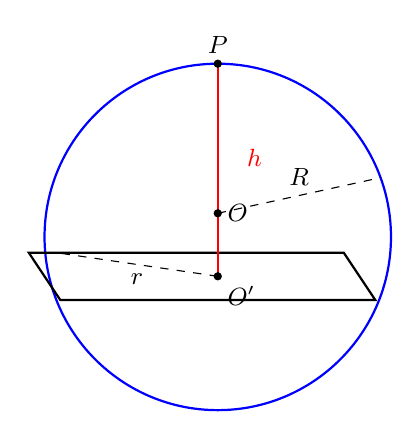
\begin{tikzpicture}[scale=1]
    \draw[thick, blue] (0,0) circle (2.2);
    \draw[thick] (-2, -0.8) -- (2, -0.8) -- (1.6, -0.2) -- (-2.4, -0.2) -- cycle;
    \coordinate (P) at (0, 2.2);
    \coordinate (Op) at (0, -0.5);
    \coordinate (O) at (0, 0.3);
    \draw[thick, red] (P) -- (Op);
    \fill (P) circle (1.5pt) node[above] {\small $P$};
    \fill (O) circle (1.5pt) node[right] {\small $O$};
    \fill (Op) circle (1.5pt) node[below right] {\small $O'$};
    \node[red] at (0.25, 1.0) [right] {\small $h$};
    \draw[dashed] (O) -- ({2.2*cos(20)}, {2.2*sin(20)}) node[midway, above] {\small $R$};
    \draw[dashed] (Op) -- (-2.05, -0.2) node[midway, below] {\small $r$};
\end{tikzpicture}
\end{center}

\rmkb{
    \textbf{球心定位的三步走}：
    \begin{enumerate}
        \item \textbf{找一个"好"的面}——外接圆圆心能算出来的（一般选底面、或含特殊几何信息的面）；
        \item \textbf{过外接圆圆心作垂线}——球心必在此线上；
        \item \textbf{用"球心到各顶点距离相等"列方程}——常常化成 $R^2 = (h - R)^2 + r^2$ 或类似形式。
    \end{enumerate}

    \textbf{什么是"好"的面}？外接圆圆心\textbf{有显式描述}的面，常见：
    \begin{itemize}
        \item \textbf{正多边形}：圆心即中心；
        \item \textbf{直角三角形}：圆心为\textbf{斜边中点}；
        \item \textbf{等腰/等边}：由对称确定圆心位置。
    \end{itemize}
}
